\documentclass[12pt]{article}

% Sets document language to English (some british conventions in
% hyphenation). Can also handle multilingual documents.
\usepackage[british]{babel}
\usepackage{csquotes}
\usepackage{pdflscape} 
\usepackage{geometry}
\usepackage{longtable}
\usepackage{gensymb}
\usepackage{listings}
\lstset{
  tabsize=2,
  breaklines=true,
  captionpos=b,
  extendedchars=true,
  numbers=left,
  basicstyle=\ttfamily,
  commentstyle=\color{red!70!black},
  keywordstyle=\color{green!70!black},
  numberstyle=\tiny\color{black!50},
  stringstyle=\ttfamily\color{blue!50!black},
  backgroundcolor=\color{yellow!10}
}
% Uses the newer biblatex (with biber as backend) for citations and
% references. Can deal with non-ascii letters in author names.
\usepackage{biblatex}
\addbibresource{references.bib}

% Provides more maths support and the theorem environments.
\usepackage{amsmath}
\usepackage{amsthm}
\theoremstyle{plain}
\newtheorem{theorem}{Theorem}
\newtheorem{lemma}[theorem]{Lemma}
\theoremstyle{definition}
\newtheorem{definition}[theorem]{Definition}

% Font handling here is intended for LuaTeX or XeTeX engine.
% Sets the font. In this case a font similar to Times.
\usepackage{fontspec}
\setmainfont{TeX Gyre Termes}
\setmonofont{Source Code Pro}[Scale=MatchLowercase]
% Unicode math fonts
\usepackage{unicode-math}
\setmathfont{texgyretermes-math.otf}

% Some generally useful packages:
% Provides \includegraphics to insert images.
\usepackage{graphicx}
% Provides \url to insert url links.
\usepackage{url}
% Provides colour support.
\usepackage{xcolor}
% Provides tables that are aesthetically more pleasing.
\usepackage{booktabs}
% Provides more configurable itemised and enumerated lists.
\usepackage{enumitem}
% Provides environment for defining vector graphics drawings.
\usepackage{tikz}
% Provides environment for code listings.
\usepackage{listings}
\lstset{
  tabsize=2,
  breaklines=true,
  captionpos=b,
  extendedchars=true,
  numbers=left,
  basicstyle=\ttfamily,
  commentstyle=\color{red!70!black},
  keywordstyle=\color{green!70!black},
  numberstyle=\tiny\color{black!50},
  stringstyle=\ttfamily\color{blue!50!black},
  backgroundcolor=\color{yellow!10}
}
% Provides hyperlinks in the pdf. Not suitable for printed documents,
% but fine here.
\usepackage[pdfborder={0 0 0},colorlinks=true,allcolors={blue!40!black}]{hyperref}

% Load the style file (title page and declarations) for the document.
\usepackage[]{swanseaTitleUG}

% Paragraphs are typeset with a small skip between them.
\usepackage[parfill]{parskip} 

% User supplied information that appears on title page. Do edit these!
\title{ Shoulder Surfing Detection}
\author{Katie Peacey}
\studentid{2214646}
\project{Shoulder Surfing Detector}

% Table of contents only lists 2 levels.
\setcounter{tocdepth}{2}

\begin{document}
\pagenumbering{roman}

\maketitle
\studentdeclarations

\begin{frontmatterparagraph}{Abstract}
Shoulder surfing is the act of visually observing someone’s private screen interactions without their consent and remains a significant privacy concern in public and semi-public spaces. From entering passwords at ATMs to composing confidential emails on laptops in cafes, users are increasingly vulnerable to visual eavesdropping. Past work on solutions such as physical privacy screens or behavioural adjustments often require users to alter their behaviour or purchase additional hardware however these approaches frequently compromise usability, reduce screen visibility or demand constant user vigilance. This paper introduces a software-based shoulder surfing detection system developed using Python. The system uses real-time gaze tracking to identify the presence of unauthorised viewers and responds by sounding an alert and dimming the display to obscure sensitive content. The system has been designed  with the user experience in mind, so seeks to be non-intrusive and responsive to the user context indicating a strong potential for broader application across both mobile and desktop platforms.
\end{frontmatterparagraph}

% Build the table of contents page.
\tableofcontents

% These lists are optional, especially if they are empty.
\listoffigures
\listoftables
\clearpage

% Reset numeric page numbering from page 1
\pagenumbering{arabic}

\section{Introduction}
\label{sec:intro}

As mobile computing becomes more embedded in daily life, the risks associated with using devices in public spaces grow. One such risk is shoulder surfing, where an attacker visually observes private information on a user’s screen, either actively or passively (Eiband et al. 2017). With the increasing use the laptops, tablets, mitigating the risk without disrupting the users experience is  a growing concern. 

Traditional solutions like privacy screen protectors (Lian et al. 2013) and authentication methods (Passfaces, DAS), often rely on hardware or face challenges in long-term usability. There is a need for adaptive, ambient solutions that are minimally intrusive and seamlessly integrate with user behaviour.

This paper introduces a gaze-based detection system as a productive solution to shoulder surfing. Implemented in Python, the system utilizes computer vision and gaze estimation techniques to monitor the presence of faces within a device’s camera view.

The primary contributions of this research are:
-	The development and evaluation of a user-centred, software-only shoulder surfing detection tool.
-	A user-centred design approach emphasizing unobtrusive, ambient feedback.
-	Add aims here?


\section{Related Work}
\label{sec:Related Work} 

Shoulder surfing is an increasingly prevalent issue. The occurrence of shoulder surfing is not limited to malicious attacks, it also includes unintentional glances and peeking out of interest. Research by Eiband et al. (2017) demonstrates that shoulder-surfing is commonplace, especially on public transportation and in communal environments. Their study suggests that users often lack awareness of being observed and generally underestimate the risk. Similarly, studies by Aviv et al. (2017) and De Luca et al. (2014) show how attackers can retrieve PINs and passwords through observational techniques, emphasising the urgency of practical mitigation strategies.

The earliest responses to shoulder surfing have been physical: privacy filters and screen covers (Lian et al. 2013). These accessories reduced the screen’s visibility angle to deter side glances from others. However, they also reduce usability for the primary user, especially in shared or collaborative settings. Something more about physical defences... 

Something about software-based defences. For example, Wiedenbeck et al. (2005) evaluated the DAS (Draw-a-secret) approach, while Tari et al. (2006) explored PIN-entry systems that reduce predictability. Though promising, these methods often compromise efficiency and are reflected by users for being cumbersome (Kroeze & Olivier, 2008).

Computer vision techniques have gained traction for dynamic user-aware defences. Brudy et al. (2014) introduced methods to detect onlookers in the context of public displays, while Khamis et al. (2016) explored gaze-based user interfaces that adapt to attention shifts. Real-time face detection, such as YOLO (You-Only-Look-Once)(Redmon et al. 2016), provides a fast and accurate way to identify multiple individuals in a frame. Insert YOLO facts here. This will be further discussed.

Gaze interaction has been increasingly used not only for input but also for context awareness and security. Holland and Komogortsev (2012) demonstrated that haze can be used for continuous authentication, while Kumar et al. (2007) showed gaze patterns can distinguish between users. Recent work by Liu et al. (2007) investigates how gaze cues can signal environmental risks without interrupting primary tasks. Such ambient strategies align closely with Weiser and Brown’s (1996) concept of calm technology interfaces that remain in the background until needed.

Something about UX. Research by Cranor and Garfinkel (2005) and more recent works by Nappa et al. (2019) confirm that users resist tools that are overly intrusive or complex. This proves that the most effective solutions are those that operate passively, offer user control and integrate smoothly into daily workflows. Expand bitch.

Our system stands in the intersection of these lines of research. It bridges the high-performance detection with subtle, user-oriented alerts, guided by formative research in UX and informed by the limitations of past solutions.

\section{System Design}
\label{sec:system design}

\subsection{Overview of the system}
\label{sec:Overview of the system}

The proposed solution is a software-based approach that detects potential shoulder surfing by using gaze tracking. It was developed in Python with a focus of usability, responsiveness and adaptability within different environments. The solution aims to minimise user disruption by only providing feedback when a potential threat is detected.

The system uses a live video input combined with a gaze tracking algorithm to determine whether a user is being observed. The central idea is to detect multiple faces within the webcam view and compare this to the gaze direction to decide whether an unauthorised person is looking at the user’s screen. Once detected, the system triggers a response where the screen brightness is reduced, and an audio alert plays to notify the user discreetly. The user can remain in control of the system via a graphical interface with start/stop buttons and customizable settings.

\subsection{Determining an appropriate algorithm}
\label{Determining an appropriate algorithm}

With the focus of the project being the user experience instead of the direct detection, we researched different machine learning algorithms that could be used to effectively identify more than one person within the webcam view at once.

\subsubsection{YOLO (You Only Look Once)}
During the initial planning of this project, an object detection algorithm called YOLO \textcolor{red}{ref here} was identified as a possible solution. 
YOLO (You Only Look Once) is an object detection algorithm produced in 2015 by Redmon et al. which uses bounding boxes to predict the probability of what each object is \cite{redmon_you_2016}. The algorithm has been trained using the ImageNet dataset \cite{noauthor_imagenet_nodate} and can detect from traffic lights to toilets. The YOLO model splits each image into a grid and produces bounding boxes for each cell, a class probability is listed, and a confidence score is calculated. The class probability is the likelihood that each object belongs to each class (e.g. bottle, person, chair) and the confidence is the likelihood that there is an object in that cell \cite{redmon_you_2016}. An overall confidence score can then be calculated and produced to the user using the formula: 
\[
  Confidence = Object Confidence Score \times Class Probability
\]
The confidence will then be listed between 1 and 0, 0 being no object found.

During initial planning, the algorithm was imported into Python and connected to the device’s camera. It was verified that YOLO processes images at 45 frames per second \cite{redmon_you_2016} meaning a passer-by should be detected in the time they walk past the screen. Figure~\ref{fig:figure1} shows the code being run on an Apple MacBook (720p FaceTime HD camera) to demonstrate its ability to detect more than one person at different distances and angles.

Images 1 and 2 demonstrate how more than one person can be identified at once – something that the shoulder surfing detector needs to do. Facial features do not need to be present to be identified correctly. Image 3 shows the main user with the onlooker stood approximately 6 meters behind. This resulted in an average confidence score of 0.95 meaning it was a strong identification.

\begin{figure}[ht]

\centering
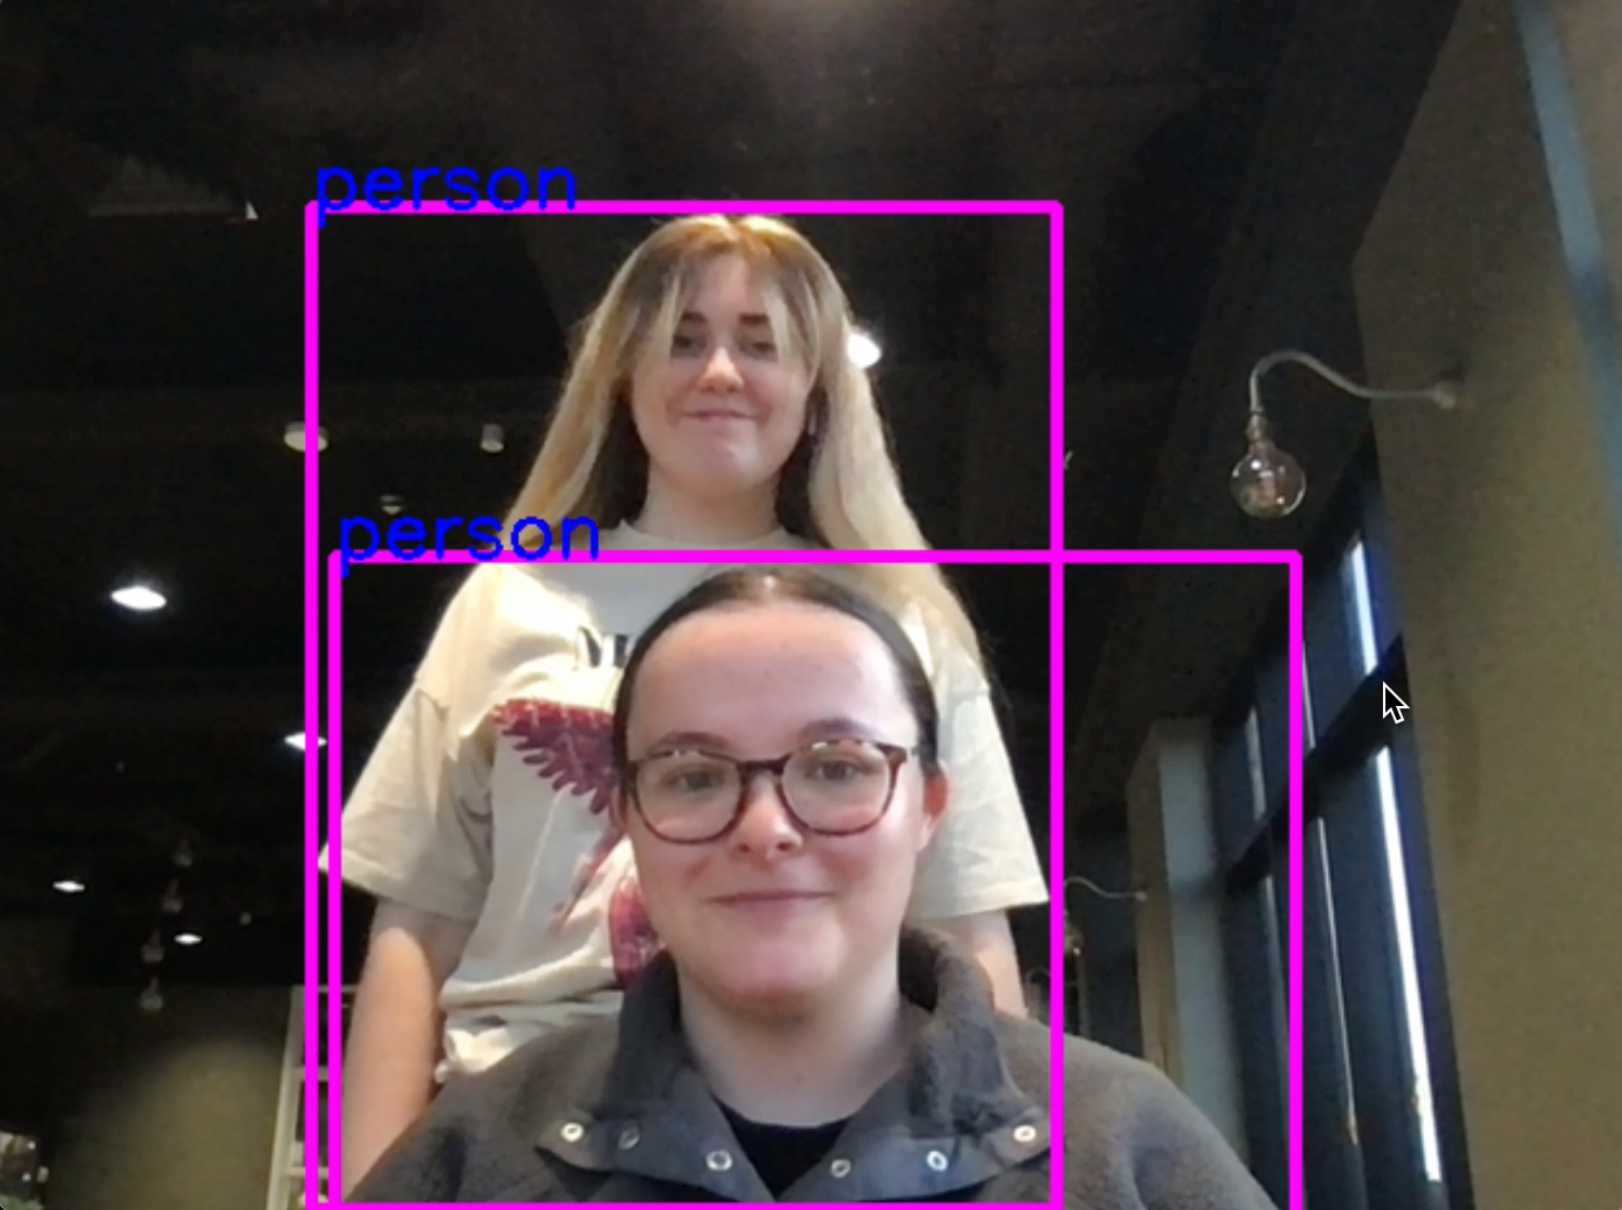
\includegraphics[width=.3\textwidth]{img/fig1-img1.png}\hfill
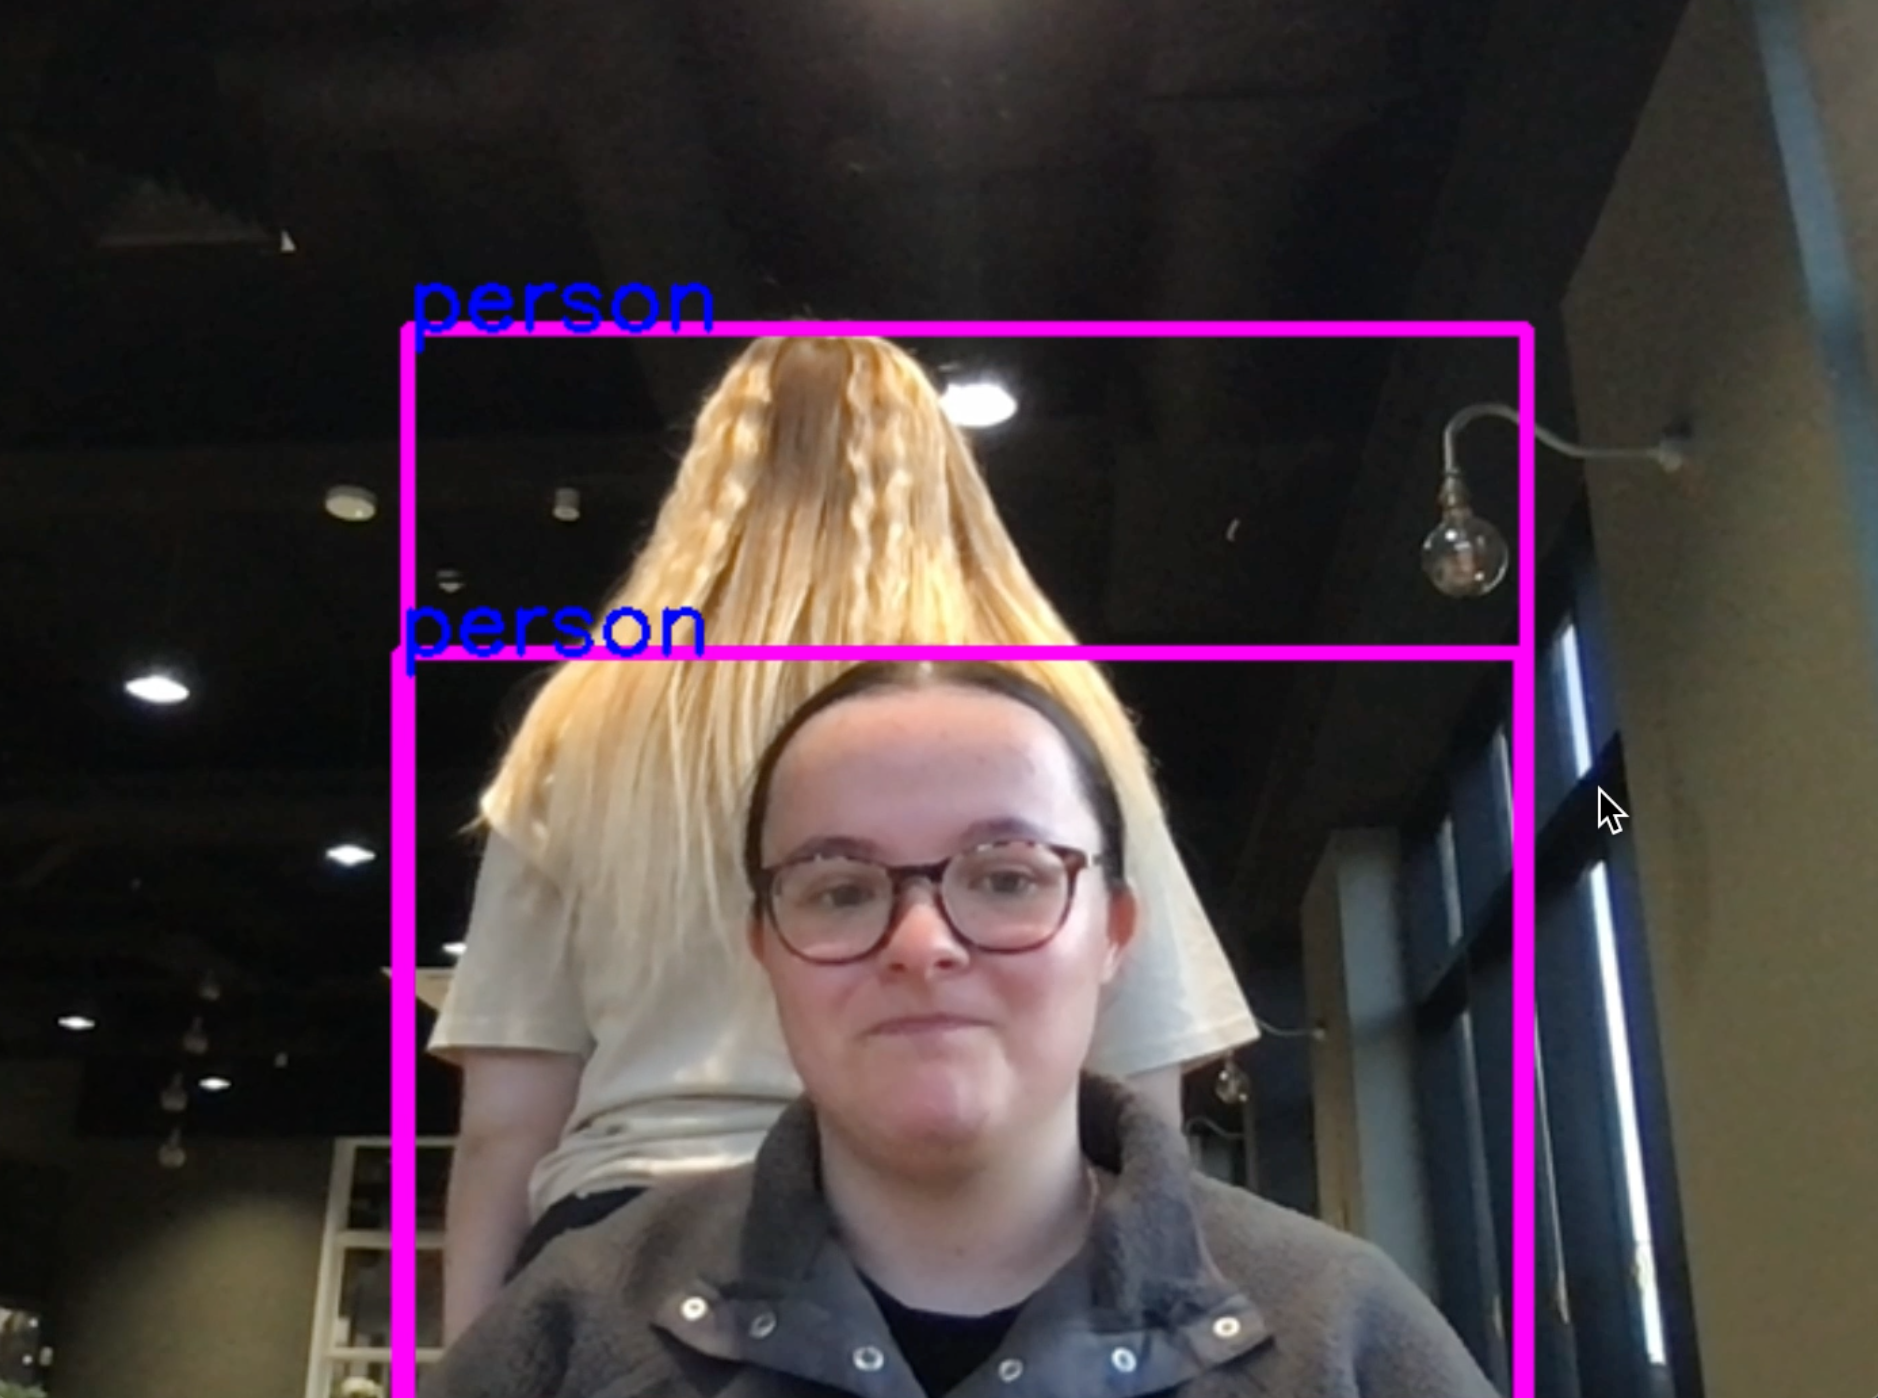
\includegraphics[width=.3\textwidth]{img/fig1-img2.png}\hfill
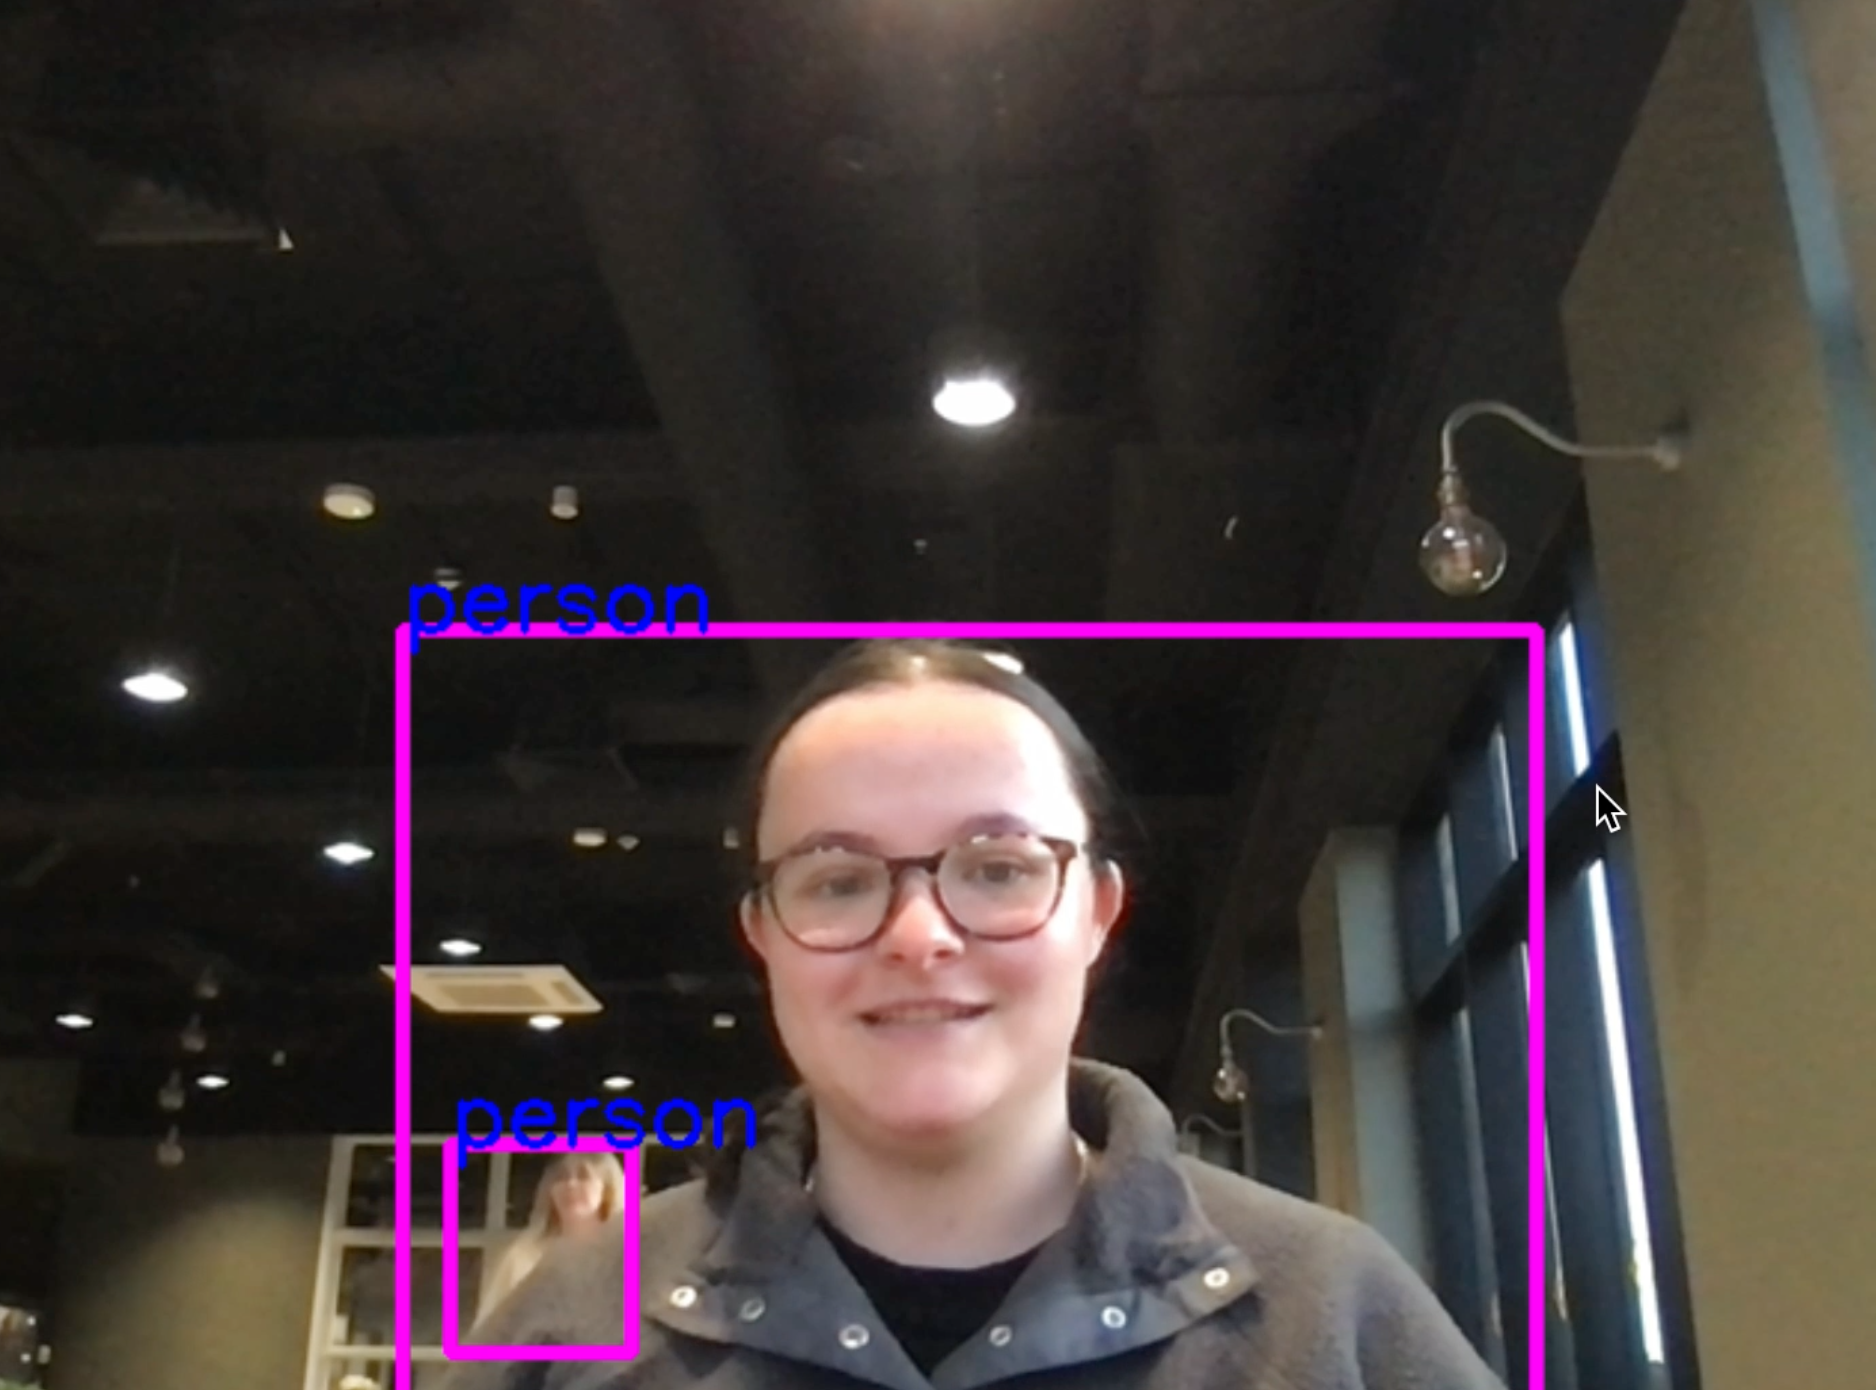
\includegraphics[width=.3\textwidth]{img/fig1-img3.png}\hfill

\caption{YOLO being used to detect more than one person in-front of the camera. The observer stands at different distances and angles to test the system.}
\label{fig:figure1}
\end{figure}

\end{document}
